% Options for packages loaded elsewhere
\PassOptionsToPackage{unicode}{hyperref}
\PassOptionsToPackage{hyphens}{url}
%
\documentclass[
]{article}
\usepackage{amsmath,amssymb}
\usepackage{lmodern}
\usepackage{iftex}
\ifPDFTeX
  \usepackage[T1]{fontenc}
  \usepackage[utf8]{inputenc}
  \usepackage{textcomp} % provide euro and other symbols
\else % if luatex or xetex
  \usepackage{unicode-math}
  \defaultfontfeatures{Scale=MatchLowercase}
  \defaultfontfeatures[\rmfamily]{Ligatures=TeX,Scale=1}
\fi
% Use upquote if available, for straight quotes in verbatim environments
\IfFileExists{upquote.sty}{\usepackage{upquote}}{}
\IfFileExists{microtype.sty}{% use microtype if available
  \usepackage[]{microtype}
  \UseMicrotypeSet[protrusion]{basicmath} % disable protrusion for tt fonts
}{}
\makeatletter
\@ifundefined{KOMAClassName}{% if non-KOMA class
  \IfFileExists{parskip.sty}{%
    \usepackage{parskip}
  }{% else
    \setlength{\parindent}{0pt}
    \setlength{\parskip}{6pt plus 2pt minus 1pt}}
}{% if KOMA class
  \KOMAoptions{parskip=half}}
\makeatother
\usepackage{xcolor}
\IfFileExists{xurl.sty}{\usepackage{xurl}}{} % add URL line breaks if available
\IfFileExists{bookmark.sty}{\usepackage{bookmark}}{\usepackage{hyperref}}
\hypersetup{
  pdftitle={Natural Computing CW},
  pdfauthor={Ahmed Ali},
  hidelinks,
  pdfcreator={LaTeX via pandoc}}
\urlstyle{same} % disable monospaced font for URLs
\usepackage[margin=1in]{geometry}
\usepackage{longtable,booktabs,array}
\usepackage{calc} % for calculating minipage widths
% Correct order of tables after \paragraph or \subparagraph
\usepackage{etoolbox}
\makeatletter
\patchcmd\longtable{\par}{\if@noskipsec\mbox{}\fi\par}{}{}
\makeatother
% Allow footnotes in longtable head/foot
\IfFileExists{footnotehyper.sty}{\usepackage{footnotehyper}}{\usepackage{footnote}}
\makesavenoteenv{longtable}
\usepackage{graphicx}
\makeatletter
\def\maxwidth{\ifdim\Gin@nat@width>\linewidth\linewidth\else\Gin@nat@width\fi}
\def\maxheight{\ifdim\Gin@nat@height>\textheight\textheight\else\Gin@nat@height\fi}
\makeatother
% Scale images if necessary, so that they will not overflow the page
% margins by default, and it is still possible to overwrite the defaults
% using explicit options in \includegraphics[width, height, ...]{}
\setkeys{Gin}{width=\maxwidth,height=\maxheight,keepaspectratio}
% Set default figure placement to htbp
\makeatletter
\def\fps@figure{htbp}
\makeatother
\setlength{\emergencystretch}{3em} % prevent overfull lines
\providecommand{\tightlist}{%
  \setlength{\itemsep}{0pt}\setlength{\parskip}{0pt}}
\setcounter{secnumdepth}{-\maxdimen} % remove section numbering
\usepackage{caption}
\usepackage{multirow}
\usepackage{float}
\restylefloat{table}
\usepackage{adjustbox}
\usepackage{float}
\usepackage{booktabs}
\usepackage{longtable}
\usepackage{array}
\usepackage{multirow}
\usepackage{wrapfig}
\usepackage{colortbl}
\usepackage{pdflscape}
\usepackage{tabu}
\usepackage{threeparttable}
\usepackage{threeparttablex}
\usepackage[normalem]{ulem}
\usepackage{makecell}
\usepackage{xcolor}
\ifLuaTeX
  \usepackage{selnolig}  % disable illegal ligatures
\fi

\title{Natural Computing CW}
\author{Ahmed Ali}
\date{}

\begin{document}
\maketitle

\newpage

\hypertarget{natural-algorithms-analysis}{%
\section{Natural Algorithms
Analysis}\label{natural-algorithms-analysis}}

In this report, I analyze the optimzaiton of two objective functions
using novel natural algorithms to analyse the behaviour of the fitness
envioremnet. This report summarizes the analysis of Standard Particle
Swarm Optimzation e.g.''PSO'' Analysis, Scaled PSO, Hetreogenous PSO ,
Differential Evolution and Genetic Programming.

\begin{longtable}[]{@{}lrll@{}}
\toprule
Name & Dim & Range & Optimal.Minimum \\
\midrule
\endhead
Sphere & 3 & {[}-5.12,5.12{]} & (0,0,0) \\
Rastrigin & 3 & {[}-5.12,5.12{]} & (0,0,0) \\
\bottomrule
\end{longtable}

A Sphere function \(f(x_i,...,x_d)=\sum_{i=1}^d x_i^2\) in a 3D-Plane is
a continuous, convex and uni-modal function that has a one global
minimum and a rastrigin function
\(f(x_i,...,x_d) = 10d + \sum_{i=1}^d(x_i^2-10cos(2\pi x_i))\) in a
3D-plane is a Continuous, non-convex and multi-modal function that has a
hill like local minima and one global minimum, Graphically as follows :

\begin{figure}[H]

{\centering 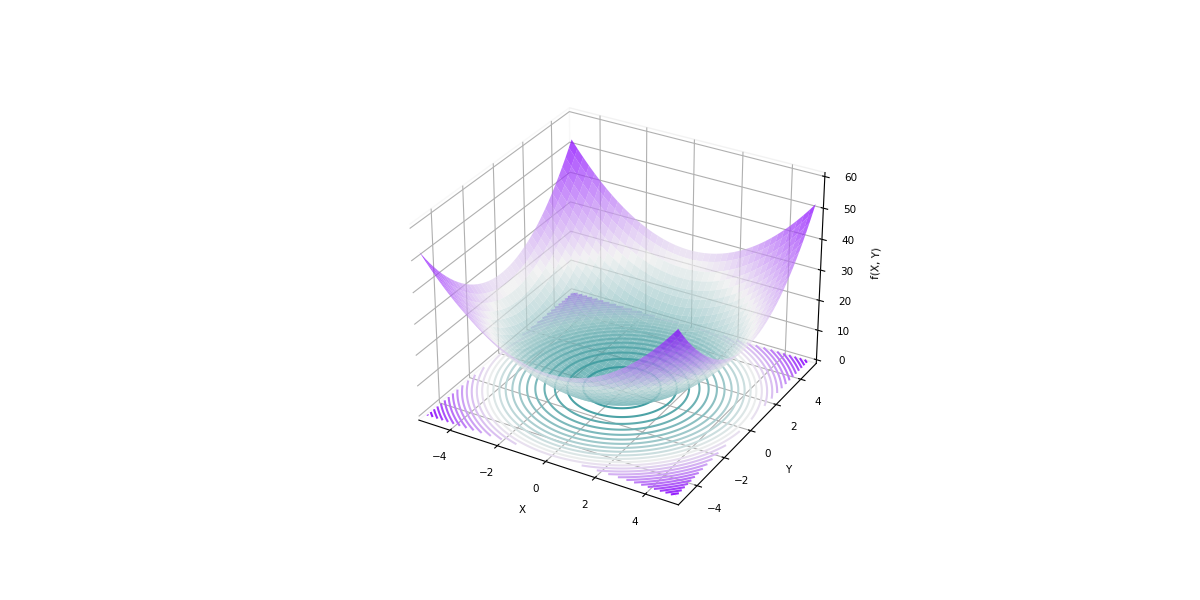
\includegraphics[width=0.8\linewidth,height=0.8\textheight,]{Particle_Swarm_Optimization-main/src/Sphere/sphere} 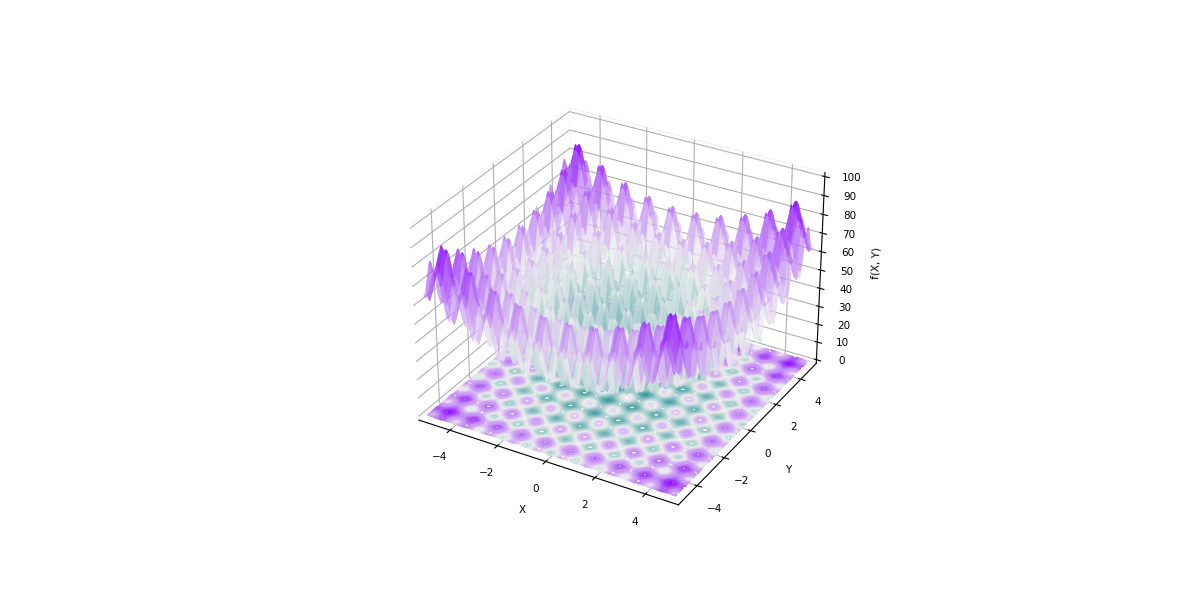
\includegraphics[width=0.8\linewidth,height=0.8\textheight,]{Particle_Swarm_Optimization-main/src/Rastrigin/rastrigin} 

}

\caption{Sphere and Rastrigin Function}\label{fig:unnamed-chunk-2}
\end{figure}

\newpage

\hypertarget{particle-swarm-optimization}{%
\section{Particle Swarm
Optimization}\label{particle-swarm-optimization}}

Analysis of particle's Swarm relies on the trade off between exploration
and exploitation which is governed by three coefficient control which
are the inertia `\(w\)', cognitive `\(c_1\)' and social `\(c_2\)'
coefficients, these are the main attributes that control the movement
and how fast the particle's find a solution . At each iteration the
cognitive and social accelerations are adjusted by the weights `\(r_1\)'
and `\(r_2\)', where these values are unique for each particle and
iteration. Inertia allows us to define the swarm change in direction.
The capacity of the group to be impacted by the best individual
solutions discovered across the iterations is defined using the
`\(c_1\)' hyperparameter. The capacity of the group to be impacted by
the best overall solution discovered during iterations is defined by the
hyperparameter `\(c_2\)'. More over that how fast an optimal solution is
reached also may depend on number of paritcles in a swarm or the search
dimension.

In reference to J. Kennedy and R. Eberhart\footnote{J. Kennedy and R.
  Eberhart, ``Particle swarm optimization,'' Proceedings of ICNN'95 -
  International Conference on Neural Networks, 1995, pp.~1942-1948
  vol.4, doi: 10.1109/ICNN.1995.488968.} work, the notations used shall
be the same as follows :

\begin{table}[H]
\centering\begingroup\fontsize{8}{10}\selectfont

\begin{tabular}{l|l}
\hline
Parameters & Description\\
\hline
N & Number of Particles in a Population\\
\hline
d & Number of Dimensions\\
\hline
Tmax & Maximum Number of Evaluation\\
\hline
T & Number of Iterations\\
\hline
\end{tabular}
\endgroup{}
\end{table}

\begin{table}[H]
\centering\begingroup\fontsize{8}{10}\selectfont

\begin{tabular}{l|l}
\hline
Hyper.parameter & Description\\
\hline
w & Inertia\\
\hline
c1 & Social Compoonent\\
\hline
c2 & Cognitive Component\\
\hline
\end{tabular}
\endgroup{}
\end{table}

\hypertarget{graphical-and-analytical-convergence-analysis}{%
\subsection{Graphical and Analytical Convergence
Analysis}\label{graphical-and-analytical-convergence-analysis}}

To visualize the influence of the inertia coefficient `\(w\)'. We can
see that the lower the `\(w\)' the stronger the convergence and the
higher the `\(w\)' until it approaches 1 the stronger the divergence,
contrarily a low value of `\(w\)' facilitates the exploitation of the
best solution however a high value of `\(w\)' facilitates the
exploration around those solutions.

\begin{center}\includegraphics[width=0.75\linewidth,height=0.15\textheight,]{../../../../../../Desktop/Screen Shot 2022-11-21 at 6.17.47 PM} \end{center}

\begin{figure}[H]

{\centering 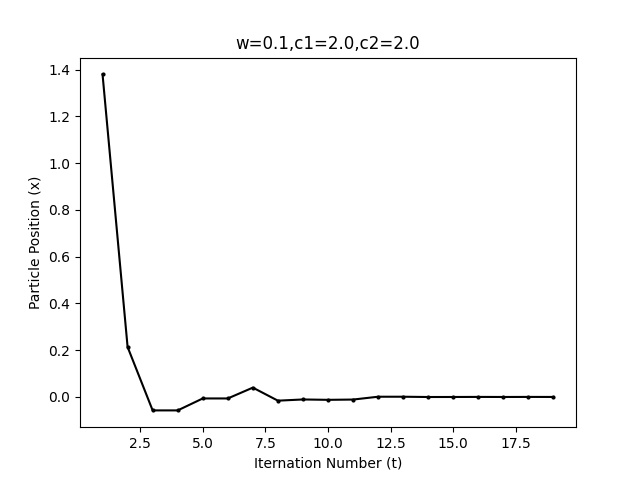
\includegraphics[width=0.3\linewidth,height=0.1\textheight,]{Particle_Swarm_Optimization-main/Optimization Data/Plots/w0.1_sphere} 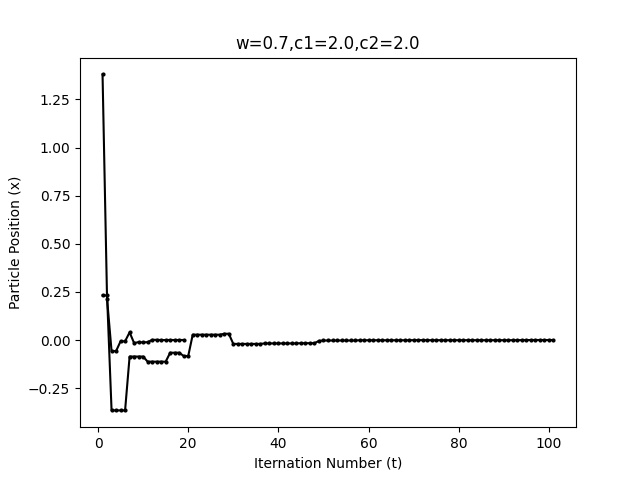
\includegraphics[width=0.3\linewidth,height=0.1\textheight,]{Particle_Swarm_Optimization-main/Optimization Data/Plots/w0.7_sphere} 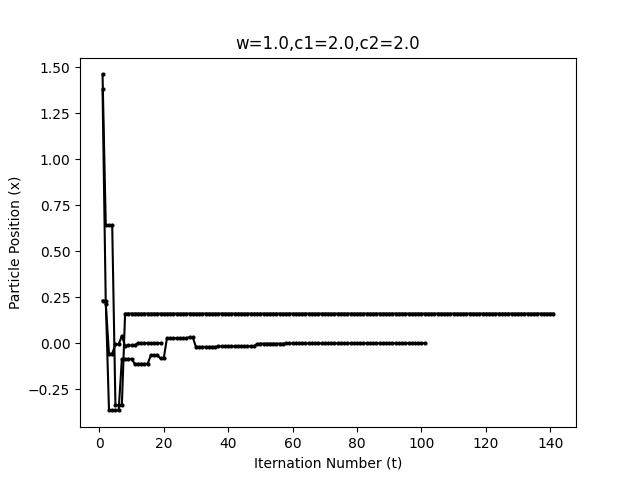
\includegraphics[width=0.3\linewidth,height=0.1\textheight,]{Particle_Swarm_Optimization-main/Optimization Data/Plots/w1.0_sphere} 

}

\caption{Sphere Convergence Fixed 'c1' and 'c2' \label{fig:sphereconvergencefc1c2}}\label{fig:sphereconvergencefc1c2 }
\end{figure}

Shown in Figure \ref{fig:sphereconvergencefc1c2}, when \(w=0.1\) we can
see that particles are allowed to explore simultaneously and freely
around search space as there direction changes at an instantaneous rate,
since there is one global minimum as soon as the fitness value decreases
drastically the swarm immediately moves toward that single best fitness
value of a particle. Meanwhile when \(w=0.7\) the inertia component of
the velocity forces the individual particles to still explore around the
minimum found by the swarm to avoid falling directly into a local
minimum until a termination criteria is met or the maximum iteration is
reached, meanwhile when \(w=1.0\) the particle's motion is entirely
influenced by the previous motion which is the initial assigned velocity
and keeps on going into the same direction. A low value of w indicates a
Non-harmonic convergence of particles as we increase the inertia the
movement goes from a harmonic low conergence scheme to high convergence
until a value of \(w=1\) is reached in which the particles in the swarm
diverge.

\begin{center}\includegraphics[width=0.75\linewidth,height=0.15\textheight,]{../../../../../../Desktop/Screen Shot 2022-11-21 at 6.15.44 PM} \end{center}

\begin{figure}[H]

{\centering 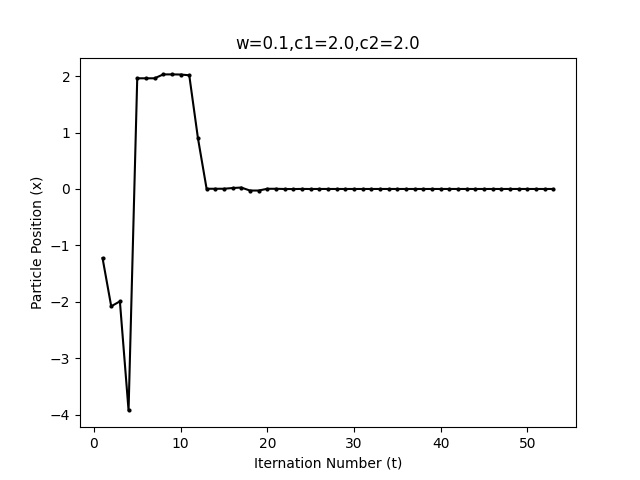
\includegraphics[width=0.3\linewidth,height=0.1\textheight,]{Particle_Swarm_Optimization-main/Optimization Data/Plots/w0.1_rastrigin} 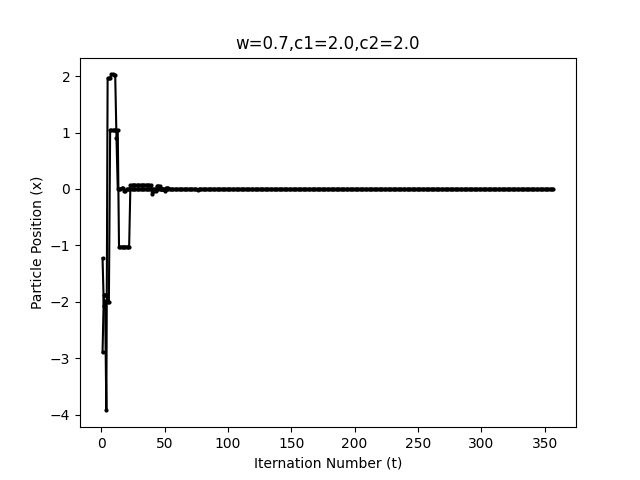
\includegraphics[width=0.3\linewidth,height=0.1\textheight,]{Particle_Swarm_Optimization-main/Optimization Data/Plots/w0.7_rastrigin} 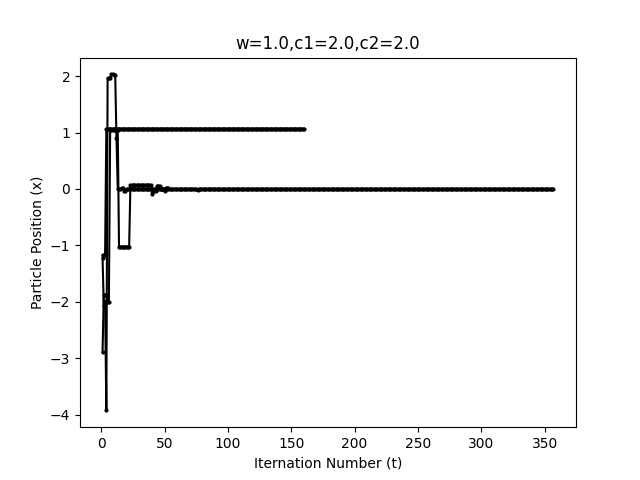
\includegraphics[width=0.3\linewidth,height=0.1\textheight,]{Particle_Swarm_Optimization-main/Optimization Data/Plots/w1.0_rastrigin} 

}

\caption{Rastrigin Convergence Fixed 'c1' and 'c2' \label{fig:rastriginconvergencefc1c2}}\label{fig:rastriginconvergencefc1c2}
\end{figure}

Shown in Figure \ref{fig:rastriginconvergencefc1c2}, when \(w=0.1\) we
can see that particles are allowed to explore simultaneously and freely
around search space as there direction changes at an instantaneous rate
but this selection of low value of inertia forces the swarm to fall into
a local minimum instead of the actual global minimum. Meanwhile when
\(w=0.7\) the inertia component of the velocity forces the individual
particles to still explore around the minimum found by the swarm to
avoid falling directly into a local minimum until a termination criteria
is met or the maximum iteration is reached we can see that the swarms do
move as a group around the global minimum until reached, meanwhile when
\(w=1.0\) the particle's motion is entirely influenced by the previous
motion which is the initial assigned velocity and keeps on going into
the same direction. The motion of the particles with low inertia start
with a harmonic low convergence motion to a harmonic high convergence as
we increment the value of w note that when \(w=1.0\) the drawbacks is
that the particles fall into a local minimum too.

\newpage

To visualize the influence of the social and cognitive coefficient, I
chose the extremes of coefficients c1 and c2 and purposefully selected a
very small coefficient of w to show the effects. We can see that how the
particles are more individualistic when \(c_1\) is high, hence there is
no convergence because each particle is only focused on its own best
solution. In contrast, the particles in the swarm are more influenced
cooperatively by each other best solutions when \(c_2\) is high, we can
also see that the exploitation of the best global solution is dominated
over the exploration.

\begin{center}\includegraphics[width=0.75\linewidth,height=0.15\textheight,]{../../../../../../Desktop/Screen Shot 2022-11-21 at 6.18.33 PM} \end{center}

\begin{figure}[H]

{\centering 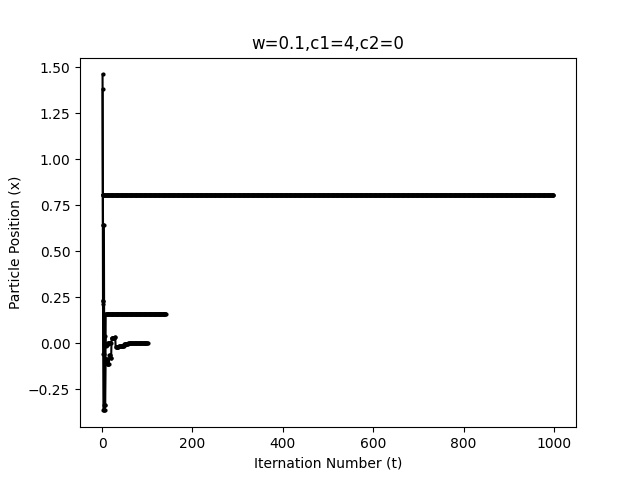
\includegraphics[width=0.3\linewidth,height=0.1\textheight,]{Particle_Swarm_Optimization-main/Optimization Data/Plots/c14c20_sphere} 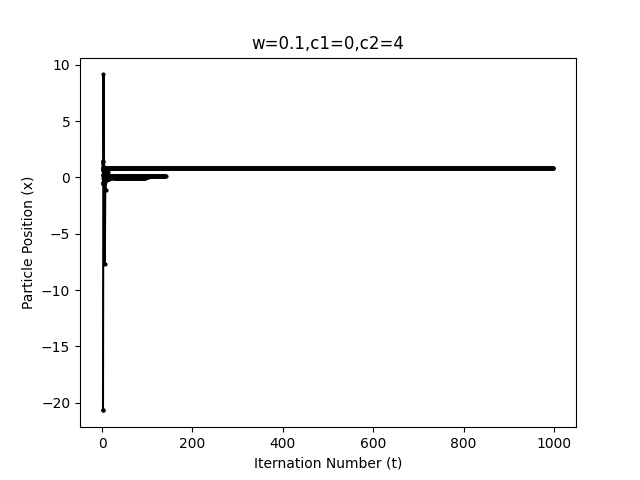
\includegraphics[width=0.3\linewidth,height=0.1\textheight,]{Particle_Swarm_Optimization-main/Optimization Data/Plots/c10c24_sphere} 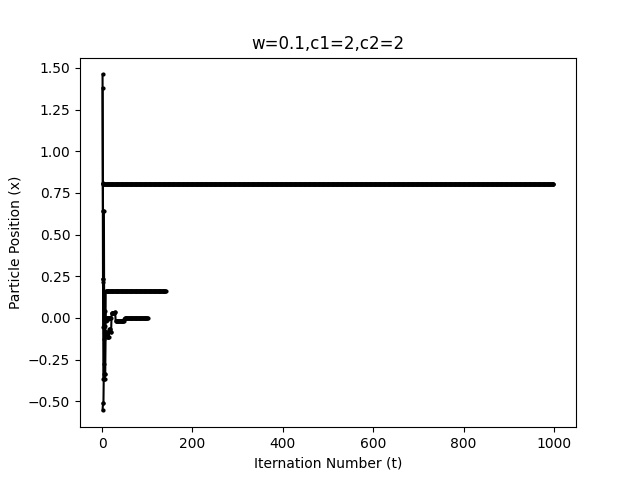
\includegraphics[width=0.3\linewidth,height=0.1\textheight,]{Particle_Swarm_Optimization-main/Optimization Data/Plots/c12c22_sphere} 

}

\caption{Sphere Convergence Fixed Inertia \label{fig:sphereconvergencefw}}\label{fig:sphereconvergencefw}
\end{figure}

Shown in Figure \ref{fig:sphereconvergencefw}, when
\(c_1=4.0\: c_2=0.0\) the particles are only attracted to there
individual best without socially communicating between each other in the
swarm the solution often would be the closest particle to the global
minimum position. When \(c_1=0.0\: c_2=4.0\), they are more influenced
by each other but notice how the movement keeps oscillating on the
y-axis.

\begin{center}\includegraphics[width=0.75\linewidth,height=0.15\textheight,]{../../../../../../Desktop/Screen Shot 2022-11-21 at 6.18.45 PM} \end{center}

\begin{figure}[H]

{\centering 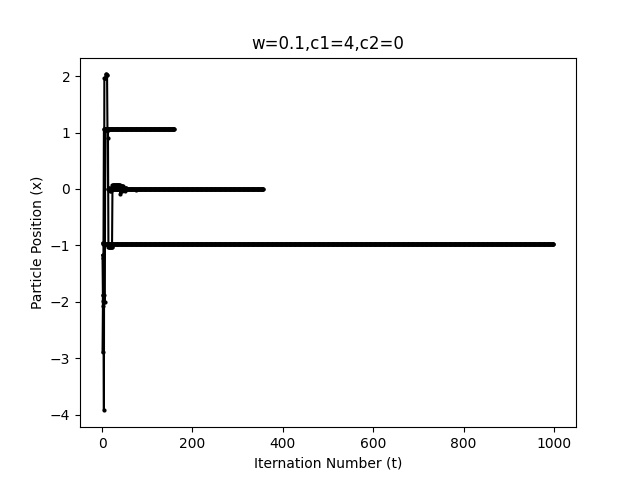
\includegraphics[width=0.3\linewidth,height=0.1\textheight,]{Particle_Swarm_Optimization-main/Optimization Data/Plots/c14c20_rastrigin} 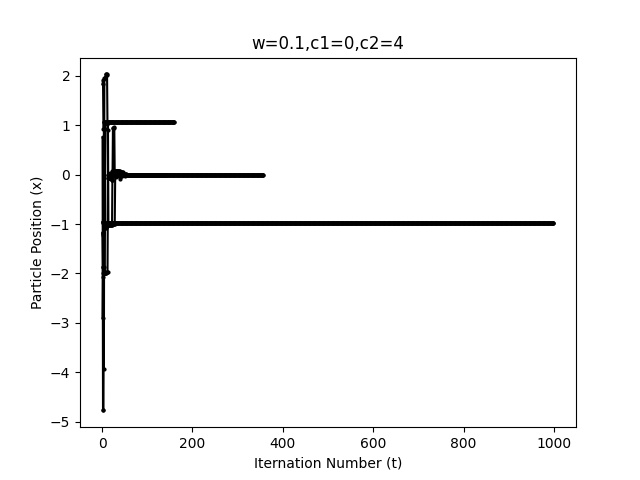
\includegraphics[width=0.3\linewidth,height=0.1\textheight,]{Particle_Swarm_Optimization-main/Optimization Data/Plots/c10c24_rastrigin} 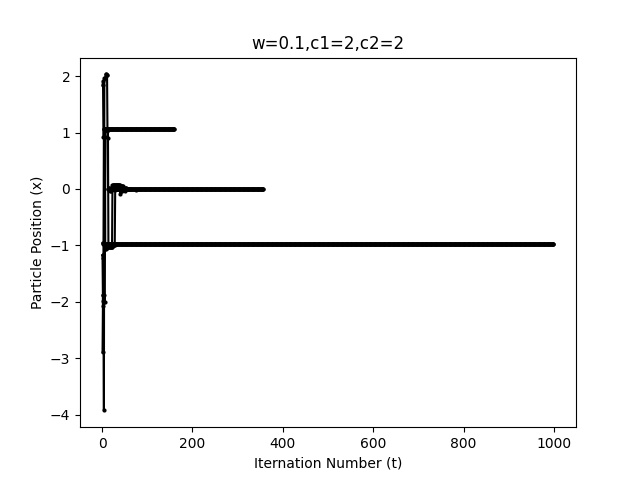
\includegraphics[width=0.3\linewidth,height=0.1\textheight,]{Particle_Swarm_Optimization-main/Optimization Data/Plots/c12c22_rastrigin} 

}

\caption{Rastrigin Convergence Fixed Inertia \label{fig:rastriginconvergencefw}}\label{fig:rastriginconvergencefw}
\end{figure}

Shown in Figure \ref{fig:rastriginconvergencefw}, When
\(c_1=4.0\: c_2=0.0\) the particles are only attracted to there
individual best without socially communicating between each other in the
swarm the solution often would be the closest particle to the global
minimum position. when \(c_1=0.0\: c_2=4.0\), they are more influenced
by each other but since the exploitation coefficient facilitates the
behavior of the swarm the swarm are practically not allowed to explore
much and they fall into a local minimum.

\newpage

\hypertarget{standard-and-auto-hyper-parameter-tuning-heuristics-of-pso}{%
\subsection{Standard and Auto Hyper-Parameter tuning heuristics of
PSO}\label{standard-and-auto-hyper-parameter-tuning-heuristics-of-pso}}

For each of the function to be optimized we adapted the following
fitness and termination criterion, an optimal solution is found if the
fitness value of the previous and the precedding iteration have a
difference of less than or equal to \(1.0e-08\), to avoid premature
convergence the algorithm terminates if the particle position is greater
than \(1.0e+22\) or the maximum number of iteration is reached without
finding an optimal solution, which means if a particle in a swarm
diverges toward the boudaries of the search space the optimization
algorithm terminates not to return the boundary space as an optimal
solution.

The standard hyperparameters are \(w=0.7\) and \(c_1 + c_2 \geq 4\),
according to the study by M. Clerc and J. Kennedy\footnote{Clerc, M.,
  And J. Kennedy. The Particle Swarm --- Explosion, Stability, And
  Convergence In A Multidimensional Complex Space.ieee Transactions On
  Evolutionary Computation 6, No.~1 (February 2002): 58--73.} to create
a standard for Particle Swarm Optimization more accurately
\(c_1 = c_2 = 2.05\). Additionally, Yuhui\footnote{Y. H. Shi And R. C.
  Eberhart, ``a Modified Particle Swarm Optimizer,'' In Proceedings Of
  The Ieee International conferences On Evolutionary Computation, Pp.
  69--73, Anchorage, Alaska, Usa, May 1998.} were the ones who first
suggested the linear decay of the parameter \(w\).So I propose the
coefficients shown below in light of these concepts and the study of G.
Sermpinis\footnote{G. Sermpinis, K. Theofilatos, A. Karathanasopoulos,
  E. F. Georgopoulos, \& C. Dunis, Forecasting Foreign Exchange Rates
  With Adaptive Neural Networks Using Radial-basis Functions And
  Particle Swarm Optimization, European Journal Of Operational Research.}.
We want to trend towards a weak `\(c_1\)', weak `\(w\)', and strong
`\(c_2\)' to take advantage of the best outcomes after exploration by
convergent towards the global minimum. We want to start with a strong
`\(c_1\)', strong `\(w\)', and weak `\(c_2\)' to maximize the
exploration of the search space. We adapt the following flow becuase
imperical rules cant apply to all cases where some functions only have
global minimum other may have local minimum in which it requires
different set of optimal hyperparameters to converge to an optimal
solution. since high values of w oftnely forces the particles in a swarm
not to focus on scamming through the search space but to find a candaite
solution quickly enough. So, \(w^t=0.9-0.5\frac{t}{T}\),
\(c_1^t=3.5-3\frac{t}{T}\) and \(c_2^t=0.5+3\frac{t}{T}\). where t is
the current iteration of the algoirthm and T is the maximum number of
iteration.

\hypertarget{tuning-conditions}{%
\subsubsection{Tuning Conditions}\label{tuning-conditions}}

The following parameters were adapted for tuning of the hyperparameters
\(N=30\), \(d=3\), \(T_{max}=1000\), \(T=200\), randomly assigned intial
positions within search space {[}-5.12,5.12{]} and intial velocities
being restricted within \(\pm20\%\) of search space.

\hypertarget{expirmental-runs}{%
\subsubsection{Expirmental Runs}\label{expirmental-runs}}

Execution of the algorithm for 200 runs, this is because in each
evalaution per a turn our algorithm includes some random assigments of
the parameters `\(r1\)', `\(r2\)', `\(v\)', `\(x\)' which in each run
the outcome is a random value from a uniform distribution with mean of
0.5, which means at each evlaution turn different values of
hyperparameters will be given but all within the same distribution so
the consideration of certain amount of runs will facilitate all those
outcomes into the mean value becasue the mean value is more robust to
biaseness and variability instead of considering one evalution. During
the 200 expirmental runs if a set of hyperparameter converges the
fitness function then this set is considered otherwise if diverged we
negelct those set of parameters to neglect the stastical biaseness in
the measure.

\begin{table}[ht]
\centering
\begin{tabular}{llll}
\hline
Statistic & w     & c1    & c2    \\ \hline
mean      & 0.677 & 2.162 & 1.838 \\
Median    & 0.673 & 2.138 & 1.862 \\
Minimum   & 0.633 & 1.895 & 0.800 \\
Maximum   & 0.850 & 3.200 & 2.105
\end{tabular}
\centering
\begin{tabular}{llll}
\hline
Statistic & w     & c1    & c2    \\ \hline
mean      & 0.589 & 1.631 & 2.369 \\
Median    & 0.587 & 1.619 & 2.381 \\
Minimum   & 0.556 & 1.439 & 2.102 \\
Maximum   & 0.633 & 1.898 & 2.561
\end{tabular}
\caption{\label{Stathyparam}Tuned hyperparameter of PSO in Sphere and Rastrigin  Envioremnemt}
\end{table}

It can be observed that there is a certain amount of variation in the
values represented by the minimum and maximum thats why to avoid the
extremas, we should conisder a specific amount of expiremtnal runs and
get the mean value of the optimal hyperparameter. Hence, the mean
optimal hyperparameters for the sphere function are
\(w=0.677,c_1=2.162,c_2=1.838\) and for the rastrigin function are
\(w=0.588,c_1=1.631,c_2=2.369\).

The particles in sphere enviornemnt have a higher inertia value as
expected since there is only one global minimum we expect the particles
to not change direction of motion more rapidly to roam around the search
space and direct the swarm towards the center as opposed to the
rastrigin enviornemnt where there are many pitfalls for the particle to
get trapped which are the local minima we dont constraint their change
of direction for movingto the next position by a lower inertia value so
they can explore the search space more rapidly. We can see that in a
sphere enviorment the swarm has a higher ability of being influenced by
the personal best of an individual thats becuase is a uni-modal space we
want the swarm to quickly converge as soon as a global minima is found,
meanwhile for the rastrigin enviornemnt the value of `\(c_1\)' is lower
by 0.532 units this is because we want to avoid bring trapped in a local
minima. Meanwhile the rastrigin enviornement have a higher `\(c_2\)'
value by 0.531 units this is because we favor the exploitation in a
multi-modal enviornment in which particles are influenced by the global
best fitness value rather than individual .

\hypertarget{hyper-parameter-evaluation}{%
\subsubsection{Hyper-parameter
Evaluation}\label{hyper-parameter-evaluation}}

Each enviornemnt of a fitness frunction has a different set of
parameters, lets define the standard PSO parameters to be set a
\(a:\{w=0.7,c_1=2.05,c_2=2.05\}\) and the tuned hyperparaemter to be set
\(b\) were \(b:\{w=0.588,c_1=1.63,c_2=2.368\}\) for the sphere and
\(b:\{w=0.588,c_1=1.63,c_2=2.368\}\) for the rastrigin enviorneemnt.To
evalaute which set of hyperparameters are optimal for each enviornemnt,
I ran an optimization expirment with assocaited set of parameters to be
\(N=30\), \(d=3\), \(T_{max}=1000\), \(T=200\) for each set
\(a,b_1,b_2\) then calculated the Convergence rate of reaching the goal
e.g.'' Converging to a global minimum per a single iteratoin of an
evalution turn'' where
\(Convergence \: Rate=\frac{|Convergence - Median \: Iteration|}{Convergence }\).
This metric show well the hyperparameter chosen lead to a convergence
into the global minimum over the median number of iteration , a higher
metric indicates that the chosen hyperparameter suits the fitness
function envionremnt to avoid termination criterion either diverging or
not finding an optimal solution, this rate is per every iteration of
evlaaution. Since both paraemter sets are near optimal conditions
considering convergence rate per every evaluation turn would be
pointless because both parameter sets would then have a value between
\([95\%,99.95\%]\) since for every evalaution turn e.g.''T'' all the
results that were produced are either 190 or 199 out of the 200
evlauation turns were convergent.

\begin{table}[h]
\centering
\begin{tabular}{p{0.65cm}p{0.65cm}p{0.65cm}p{0.65cm}p{0.65cm}p{0.65cm}p{0.65cm}p{0.65cm}p{0.65cm}p{0.65cm}p{0.65cm}p{0.65cm}p{0.65cm}p{0.65cm}p{0.65cm}p{0.65cm}p{0.65cm}}
\cline{1-14}
\multicolumn{14}{c}{Hyper-Parameter Evaluation}                                                                                   &  &  \\ \cline{1-14}
Function &
  \multicolumn{1}{c}{N} &
  \multicolumn{8}{c}{Algorithm Iteration} &
  \multicolumn{2}{c}{Convergence} &
  \multicolumn{2}{c}{Convergence Rate} &
  \multicolumn{2}{c}{} \\ \cline{3-10}
 &
  \multicolumn{1}{c}{} &
  \multicolumn{2}{l}{Average} &
  \multicolumn{2}{l}{Median} &
  \multicolumn{2}{l}{Minimum} &
  \multicolumn{2}{c}{Maximum} &
   &
   &
   &
   &
   &
   \\ \cline{3-14}
&    & Set a & Set b & Set a & Set b & Set a & Set b & Set a & Set b & Set a & Set b & Set a  & Set b  &  &  \\ \cline{1-14}
\multicolumn{1}{c}{Sphere} & 30 & 114   & 89    & 111   & 90    & 59    & 30    & 192   & 136   & 199   & 199   & 49.7\% & 54.7\% &  &  \\
Rastrigin                  & 30 & 345   & 188   & 345   & 190   & 227   & 131   & 481   & 261   & 190   & 199   & 73.3\% & 95.4\% &  &  \\
                        
\end{tabular}
\caption{\label{Eval}Evaluation of PSO Hyperparameter in Sphere and Rastrigin Envioremnemt}
\end{table}

Based on the evaluation ilustrated, the rastrigin envionremnt is more
optimal for particles with tuned hyperparemter with an out-preformance
of 13.8\% in success over standard hyperparaemter, while the sphere
enviornemnt is more optimal for particles with standard hyperparameter
out preforming thetuned hyperparameter by 13.7\%.

\newpage

\hypertarget{scaling-of-particle-swarm-optimizaiton-algorithm}{%
\subsection{Scaling of Particle Swarm Optimizaiton
Algorithm}\label{scaling-of-particle-swarm-optimizaiton-algorithm}}

How fast the optimal solution is obtained in terms of time complexity
e.g.''iterations''?, do more particles in swarm mean more noise?, we
either iterate the number of particles \(N\), the search space dimension
\(d\), or the total number of fitness evaluations \(T\) per run are
iterated for the testing conditions, to answer the introduced question
the main parameter is the number of particles.The following parameters
were adapted for evalauting PSO algorithm \(N\in\{30,60,90\}\), \(d=3\),
\(T_{max}=1000\), \(T=200\) and randomly assigned intial positions
within search space e.g.''{[}-5.12,5.12{]}'' and inital velocities being
restricted within \(\pm20\%\) of search space.

\hypertarget{perfromance-evalaution}{%
\subsubsection{Perfromance Evalaution}\label{perfromance-evalaution}}

Adapting the standard and tuned hyperparameters sets , which are to be
set \(a:\{w=0.7,c_1=2.05,c_2=2.05\}\) and the tuned hyperparaemters to
be set
\(b:\{w=0.588,c_1=1.63,c_2=2.368\},\{w=0.588,c_1=1.63,c_2=2.368\}\). To
evalaute the affect of number of particles in a swarm the perfromance
criterion that is adapted is the number of function evalautions,
\(Evaluation=\frac{N * Median\: Iteration }{\: Convergence \:Rate }\)
and the convergence rate
\(Convergence \: Rate=\frac{|Convergence - Median \: Iteration|}{Convergence }\).
The number of fitness evaluations was selected as theperformance
criteria becuase itt considers the quantity of particles, quantity of
algorithm iterations, and convergence rate as in Table 2. The metric
showndefines how well the hyperparameter chosen lead to a convergence
into the global minimum over the median number of iteration , a lower
metric indicates that the chosen hyperparameter suits the fitness
function envionremnt to avoid termination criterion either diverging or
not finding an optimal solution.The convergence rate helps us determine
which parameter and hyperparameter settings best suit a certain
environement being evalauted.

\begin{table}[h]
  \centering
  \resizebox{5.0in}{8.0in}{%
  \begin{tabular}{p{0.1cm}p{0.1cm}p{0.55cm}p{0.55cm}p{0.55cm}p{0.55cm}p{0.55cm}p{0.55cm}p{0.55cm}p{0.55cm}p{0.55cm}p{0.55cm}p{0.55cm}p{0.1cm}p{0.55cm}p{0.55cm}}
\hline
\multicolumn{16}{c}{Scaling Evalaution}                                                                                                            \\ \hline
Function &
  \multicolumn{1}{c}{N} &
  \multicolumn{8}{c}{Algorithm Iteration} &
  \multicolumn{2}{c}{Convergence} &
  \multicolumn{2}{c}{Convergence Rate} &
  \multicolumn{2}{c}{Evalaution} \\ \cline{3-10}
 &
  \multicolumn{1}{c}{} &
  \multicolumn{2}{l}{Average} &
  \multicolumn{2}{l}{Median} &
  \multicolumn{2}{l}{Minimum} &
  \multicolumn{2}{c}{Maximum} &
   &
   &
   &
   &
   &
   \\ \cline{3-16} 
                           &    & Set a & Set b & Set a & Set b & Set a & Set b & Set a & Set b & Set a & Set b & Set a  & Set b   & Set a & Set b \\ \hline
\multicolumn{1}{c}{\multirow{3}{*}{Sphere}} &
  30 &
  114 &
  89 &
  111 &
  90 &
  59 &
  30 &
  192 &
  136 &
  199 &
  199 &
  49.7\% &
  54.7\% &
  3437 &
  2683 \\
\multicolumn{1}{c}{}       & 60 & 88    & 71    & 86    & 71    & 49    & 37    & 124   & 97    & 199   & 199   & 56.8\% & 64.3\%  & 5306  & 4281  \\
\multicolumn{1}{c}{}       & 90 & 78    & 63    & 79    & 65    & 51    & 38    & 122   & 83    & 199   & 199   & 60.3\% & 67.3\%  & 7055  & 5698  \\
\multirow{3}{*}{Rastrigin} & 30 & 345   & 188   & 345   & 190   & 227   & 131   & 481   & 261   & 190   & 199   & 73.3\% & 95.4\%  & 10894 & 5668  \\
                           & 60 & 293   & 156   & 296   & 155   & 188   & 121   & 374   & 204   & 195   & 199   & 51.7\% & 77.8\% & 18030 & 9407  \\
                           & 90 & 272   & 142   & 272   & 143   & 182   & 113   & 356   & 172   & 197   & 199   & 38.1\% & 71.9\%  & 24852 & 12844
\end{tabular}%
}
\caption{\label{EvalPSO} Evalautionof PSO in Sphere and Rastrigin  Envioremnemt}
\end{table}

For the sphere enviornement, as we increase hte number of particles in
the swarm lower iterations are required to converge this is because more
aprticles occupy the search space which leads to a higher convergence
rates increasing `N' by 60 in swarm leads to a mean increase of 11\% in
convergence rate for both parameter sets, furthermore higher onvergence
rates increases the overall evalaution criteria. Parameter set b leads
to higher convergence rates than paraemter set a, furthermore parameter
set b requires less iterations for the aglroithm which implies less
evalautions per turn hence low time complexity, in which the auto-tuned
hyperparaemters are more suitable in this enviorement. For the rastrigin
enviornement, as we increase the number of particles in the swarm lower
iterations are required to converge this is because more aprticles
occupy the search space note that this leads to a lower convergence
rates because particles in this enviorenment suffer from a higher risk
of early convergence to sub-optimal solutions instead of optimnal
solutions.Moreover, parmeter set b retians a higher convergence rate as
we increase `N' but with an overall decreasing trend, parameter set a
leads to lower convergence rate by 35.2\% as we increase `N' from 30 tom
90. Both enviornement have different outcomes the number of iterations
in sphere funciton is lower by about 65\% for convergence thats becuase
due to the convexity of the enviornemtns, for different parameters as
with sphere as `N' increase convergence rate increases while the
rastrigin function forces a decrease in outcome due to the hgier risk of
pitfalling into a local minima. Since number of evalaution per turn is
higher for rastrigin enviorneemnt its time complexity for convergence of
algorithm is typically higher than sphere envionremnt thats because we
require more comptuational resources and time to compute comparisions of
personal and global fitness values.

\hypertarget{effect-of-the-fitness-enviornemnt}{%
\paragraph{Effect of the fitness
enviornemnt}\label{effect-of-the-fitness-enviornemnt}}

\begin{table}[H]
\centering
\resizebox{3.0in}{!}{%
\begin{tabular}{llll}
\hline
Fitness   & Iterations & Convergence Rate & Evalaution \\ \hline
Sphere    & 83         & 58.9\%           & 4743       \\
Rastrigin & 233        & 68.0\%           & 13615     
\end{tabular}%
}
\end{table}

The optimal solution was always found in the center point or very close
to the centre of the search space, while the rastrigin function has a
several local minima the sphere has only one global minimum. The
rastigin function non-convexity leads to curvature that directs the
search towards the global minimum with pitfalls of local minima.
Although the median convergence rate is higher its out of scope of the
report to explain mathematical dynamic enviornemnt.

\hypertarget{effects-of-set-of-hyper-parameters}{%
\paragraph{Effects of set of
Hyper-parameters}\label{effects-of-set-of-hyper-parameters}}

\begin{table}[H]
 \centering
 \resizebox{3.0in}{!}{%
 \begin{tabular}{llll}
 \hline
 Hyper-Parameter & Iterations & Convergence Rate & Evalaution \\ \hline
 Set a           & 198        & 54.9\%       & 11595      \\
 Set b           & 119        & 71.9\%       & 6768      
 \end{tabular}%
 }
 \end{table}

The convergence rate of parameter set a is lower than that of set b. As
a result, for set a exploitation is preferred over search space
exploration and vice versa for set b. Number of evalautoins is lower for
paraemter set b which correpsonds to, the higher convergence rate a set
of parameter has the lower amount of evlautions are required since the
algorithm teriminates when a solution is found and the lower the
convergence rate the higher the number of iterations typically because
some expirmental runs diverge for a set of parameter.

\hypertarget{effects-of-number-of-particles-in-the-swarm}{%
\paragraph{Effects of number of particles in the
swarm}\label{effects-of-number-of-particles-in-the-swarm}}

\begin{table}[H]
\centering
\resizebox{2.5in}{!}{%
\begin{tabular}{llll}
\hline
N  & Iterations & Convergence Rate & Evalaution \\ \hline
30 & 184        & 68.3\%           & 5671       \\
60 & 143        & 62.5\%           & 9256       \\
90 & 140        & 59.4\%           & 12612     
\end{tabular}%
}
\end{table}

According to the median iteration above , increasing the number of
particles often results in fewer iterations being needed for
convergence. The convergence rate was also signficiantly decreased at
additional particles numbers in the swarm, this was anticipated since
more particles provide a more complete sampling of the search space in
which some most likley diverge to positions away from center. However,
additional particles necessitate more fitness analyses because more
number of particles means the comparision of fitness values of
individual best and global best requires more iterations. Best outcomes
were typically at 30 particles in a swarm, which resulted in a higer
convergence rate , higher iterations and fewer number of evalautions.

\hypertarget{optimal-conditions}{%
\paragraph{Optimal Conditions}\label{optimal-conditions}}

\begin{table}[H]
\centering
\resizebox{3.0in}{!}{%
\begin{tabular}{llllll}
\hline
Function  & w     & c1    & c2    & N  & Convergence Rate \\ \hline
Sphere    & 0.677 & 2.162 & 1.838 & 90 & 67.3\%           \\
Rastrigin & 0.589 & 1.631 & 2.369 & 30 & 95.4\%          
\end{tabular}%
}
\end{table}

Based on the analysis shown above , the optimal parameters and
hyperparameters for the algorithm for the sphere and rastrigin fucntions
are as follows where in sphere enviroenemnt exploration is facored and
in rastriging enviroenemnt exploitation is favored. Typically higher `N'
speeds up the convergence but for the rastrigin enviroenemnt it has
higher risk of falling into sub-optinal solutions thats why lower `N' is
preffered in the algorithm.

\newpage

\hypertarget{hetergonous-particle-swarm-analysis}{%
\subsection{Hetergonous Particle Swarm
Analysis}\label{hetergonous-particle-swarm-analysis}}

\newpage

\hypertarget{differential-evloution}{%
\subsection{Differential Evloution}\label{differential-evloution}}

\hypertarget{testing-conditions}{%
\subsubsection{Testing Conditions}\label{testing-conditions}}

The rastrigin fitness frunction has a different set of parameters, the
following parameters were adapted for evalautions number of generations
\(G_{max}=100\) Number of evalautions per turn \(T=1000\),dimension
\(d=3\), mutation rate \(F=0.48\), cross over rate \(Cr=0.4\), solutions
within search space \(Bounds=[-5.12,5.12]\). Mutation and cross over
rates were adapted based on a previous implemntaiton by Mirui
wang\footnote{mirui wang (2022). Optimization Rastrigin Function by
  Differential Evolution algorithm
  (\url{https://www.mathworks.com/matlabcentral/fileexchange/46818-optimization-rastrigin-function-by-differential-evolution-algorithm}),
  MATLAB Central File Exchange. Retrieved November 23, 2022.}.

\hypertarget{expirmental-runs-1}{%
\subsubsection{Expirmental Runs}\label{expirmental-runs-1}}

\begin{table}[H]
\centering
\resizebox{4in}{!}{%
\begin{tabular}{lllll}
\hline
N  & Generations & Convergence & Convergence Rate & Evalaution \\ \hline
30 & 100         & 73          & 73\%            & 4109       \\
60 & 100         & 81          & 81\%            & 7407       \\
90 & 100         & 92           & 92\%              & 9782      
\end{tabular}%
}
\end{table}

For each 100 evalutions experimental run we generated a population size
of population size \(N\in\{30,60,90\}\) in each DE run there were 1000
generations ,If error less than 1e-08 its considered convergence in
whcih optimal solution is found.For each of the population size the
convergence rates are 0.73,0.81,0.92 respectivley, as the number of
pupulation increase the convergence rate increases.

\begin{figure}[H]

{\centering \includegraphics[width=0.3\linewidth,height=0.1\textheight,]{../../../../../../Desktop/Screen Shot 2022-11-24 at 12.24.05 AM} \includegraphics[width=0.3\linewidth,height=0.1\textheight,]{../../../../../../Desktop/Screen Shot 2022-11-24 at 12.26.50 AM} \includegraphics[width=0.3\linewidth,height=0.1\textheight,]{../../../../../../Desktop/Screen Shot 2022-11-24 at 12.24.39 AM} 

}

\caption{Convergence of Rastrigin N=30,60 and 90 \label{fig:DEpopn30}}\label{fig:DEpopn30}
\end{figure}

Shown in Figure \ref{fig:DEpopn30}, the convergence of the different
number of population parameter as we can see that low number of
population dont have a lot if variation to evolve emanwhile as we
increase the nubmer of indivudals in population more varaition tends to
lead to higher convergence rates.

\begin{figure}[H]

{\centering \includegraphics[width=0.3\linewidth,height=0.1\textheight,]{../../../../../../Desktop/Screen Shot 2022-11-24 at 12.22.31 AM} \includegraphics[width=0.3\linewidth,height=0.1\textheight,]{../../../../../../Desktop/Screen Shot 2022-11-24 at 12.21.33 AM} \includegraphics[width=0.3\linewidth,height=0.1\textheight,]{../../../../../../Desktop/Screen Shot 2022-11-24 at 12.25.47 AM} 

}

\caption{Time-complexity versus Fitness \label{fig:speed}}\label{fig:speed}
\end{figure}

Shown above in Figure \ref{fig:DEpopn30}, fitness function value
e.g.''objective function value'' for differnet population sizes going
from 30 to 90, we can see that higher number of individuals in a
population tend to cover higher search space in which not alot of
mutations and crossovers are needed to compare the fitness values .
Lower slope at the begining of algorithmic iteration indicates that the
cinvergence rate is higher.

\hypertarget{perfromance-comparision-evalution}{%
\subsubsection{Perfromance Comparision
Evalution}\label{perfromance-comparision-evalution}}

\begin{table}[H]
\centering
\resizebox{2.5in}{!}{%
\begin{tabular}{lllll}
Algorithm            & N  & Generations & Convergence Rate & Evalaution \\ \hline
\multirow{3}{*}{PSO} & 30 & 345         & 95.4\%           & 5668       \\
                     & 60 & 293         & 77.8\%           & 9407       \\
                     & 90 & 272         & 71.9\%           & 12844      \\
\multirow{3}{*}{DE}  & 30 & 100         & 73\%             & 4109       \\
                     & 60 & 100         & 81\%             & 7407       \\
                     & 90 & 100         & 92\%             & 9782      
\end{tabular}%
}
\end{table}

\hypertarget{effects-of-number-of-individuals-in-a-population}{%
\paragraph{Effects of number of individuals in a
population}\label{effects-of-number-of-individuals-in-a-population}}

In the PSO algorithm as we increase the number of particles in a swarm,
we almost always suffer from premature-convergence into sub-optimnal
locations so then the convergence rate to the global minimum decreases,
as for the DE algorithm higher number of particles lead to more
exploration but becasue of mutation and cross over we lower the risk of
premature-convergence so the likelihood of converging is higher while
covering a much larger search space.

\hypertarget{effect-of-algorithm}{%
\paragraph{Effect of algorithm}\label{effect-of-algorithm}}

Convergence rates are higher using the DE algorithm, simply because of
the mutations and crossovers the algorithm has it provides more
varaiblity into the fitness enviroenment in terms of search space
exploration, meanwhile in PSO the comparsion of fitness values and
update of position and velocities typically leads to more successive
itertations to completley sweep out the search space. Number of
evalautions for PSO are higher because through the algoirhtm we loop
through a nested loop with 4 comparisions so the order of time
complexity becomes \(O(n)=4n^2\), in comparision in DE when three
individuals are chosen to perfrom mnutation and cross over that happens
in a one loop and fitness comparison in another so the time complexity
is given by \(O(n)=1n^2\) . Note that the time complexity is an
indicative measure that correlates with the high number of evaluations.

\newpage

\hypertarget{genetic-programming}{%
\subsection{Genetic Programming}\label{genetic-programming}}

The rastrigin function in 1-D is given by

\[
f(x)=10 + (x^2- 10cos(2\pi x)) \:\:(1)
\] which can be written in terms of weight and variables, were our
weight paremters are \(w=\{w_1,..,w_3\}\) \[
f(x)=10+w_0x^2+w_1cos(w_2x)\:\:(2)
\]

\hypertarget{data-set-generation}{%
\paragraph{Data set generation}\label{data-set-generation}}

To generate the data set with points (x,y), x are 500 data points
between {[}-5.12,5.12{]} and y are the rastrigin function values with
guassain noise \(Noise\sim(0,0.2)\) for those x values.

\begin{figure}[H]

{\centering \includegraphics[width=0.5\linewidth,height=0.2\textheight,]{../../../../../../Desktop/Screen Shot 2022-11-24 at 4.51.38 AM} 

}

\caption{2D Rastrigin Function \label{fig:DEpredict}}\label{fig:DEpredict}
\end{figure}

\hypertarget{differntial-evolution-as-gp}{%
\subsubsection{Differntial Evolution as
GP}\label{differntial-evolution-as-gp}}

I implemented a differential evolution scehma mentioned in Appendix
Algorithm 2, with mutation rate of 0.48 and convergence rate 0f 0.4 ,
with a population size of 30 and 1000 generations. The obejctive
function was the RMSE loss in predicted and actual values of restrigin
function to then solve for the weights hence get the coefficents of the
function . \(RMSE=\sqrt{\frac{\sum(y-y_{pred})}{500}}\), where \(y\) is
equation (1) and \(y_{pred}\) is equation (2).

\hypertarget{weight-of-coefficeints}{%
\paragraph{Weight of coefficeints}\label{weight-of-coefficeints}}

The wights of the coeffeicients are as follows
\(w=\{0.94910388,-9.76768436,0.4119\}\).

\begin{figure}[H]

{\centering 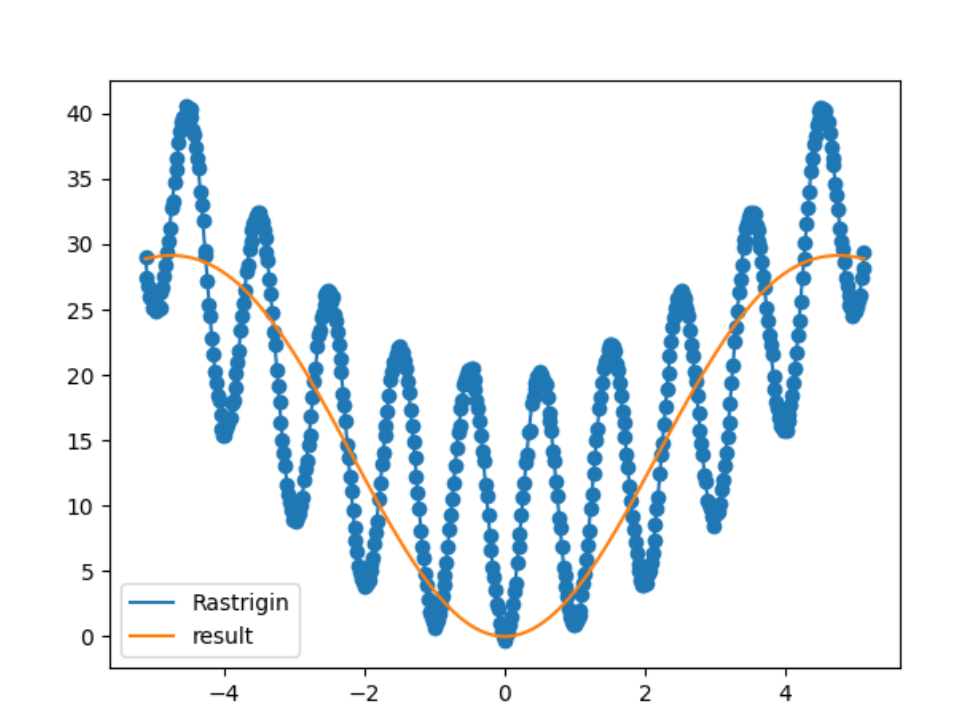
\includegraphics[width=0.5\linewidth,height=0.2\textheight,]{../../../../../../Desktop/Screen Shot 2022-11-24 at 5.23.23 AM} 

}

\caption{Result of Reproducing Function \label{fig:wegiht}}\label{fig:wegiht}
\end{figure}

\newpage

\hypertarget{acknowledgemnts}{%
\section{Acknowledgemnts}\label{acknowledgemnts}}

\begin{itemize}
\item
  Convergence analysis of PSO graphs and infromation of the flow of PSO
  was inspired from the article ``Particle Swarm Optimization (PSO)
  Visually Explained'' by Axel Thevenot,
  \url{https://towardsdatascience.com/particle-swarm-optimization-visually-explained-46289eeb2e14}
  . the overflow of the analysis was adapted from Gang Xu, Guosong Yu On
  convergence analysis of particle swarm optimization algorithm, Journal
  of Computational and Applied Mathematics, Volume 340, 1 October 2018,
  Pages 709-717 .
\item
  The Hetegounous Particel Swarm Optimization was inspired by the help
  of Chang, W.-D. (2015). A modified particle swarm optimization with
  multiple subpopulations for multimodal function optimization problems.
  Applied Soft Computing, 33, 170--182.
  \url{doi:10.1016/j.asoc.2015.04.002} .
\item
  A Guide on Differential Evolution was examined and throughly undestand
  before applying the DE analysis, by an article written by Dr.Pablo
  Rodriguez- Mier ``A tutorial on Differential Evolution in Python'' ,
  \url{https://pablormier.github.io/2017/09/05/a-tutorial-on-differential-evolution-with-python/}
  .
\end{itemize}

\newpage

\hypertarget{appendix}{%
\section{Appendix}\label{appendix}}

\hypertarget{particle-swarm-optimization-pso}{%
\subsection{Particle Swarm Optimization
(PSO)}\label{particle-swarm-optimization-pso}}

James Kennedy and Russell Eberhart first introduced Particle Swarm
Optimization e.g.''PSO''in 1995, PSO is biologically inspired
optimization routine designed to memic flocking of birds They postulated
that the swarm would benefit from the information being shared in a
social setting. Individuals members can benefit from one another's
findings and experiences anytime the resource is allocated differently
than expected, as opposed to fighting over food. ``Social contact'' is
the important phrase. Social behavior improves an individual's capacity
for adaptation, which leads to the emergence of intelligence in the
swarm. Individual adaptability and group intelligence are
interconnected.

In a search space, particle's are a variety of entities In order to
assess each particle's individual fitness, we generate a population of
particle's and use an objective function.Then, based on their individual
best location and the swarm's best location thus far, particle's are
transferred from their current to the next position. The swarm
progressively approaches an optimal position of the goal function over
generations by iterating the moves.

The resultant optimized solution is heuristic because we can never prove
the real global optimal solution can be found and it is usually not.
However, we often find that the solution found by PSO is quite close to
the global optimal.

\hypertarget{algorithm}{%
\paragraph{Algorithm}\label{algorithm}}

\(\\\)

We define a set of parameters

\begin{table}[H]
\centering\begingroup\fontsize{8}{10}\selectfont

\begin{tabular}{l|l}
\hline
Varaible & Defintion\\
\hline
i & Number of particle's\\
\hline
n & Search space dimensions\\
\hline
f(xi) & Fitness function\\
\hline
xi & particle's\\
\hline
vi & Current velocity\\
\hline
pi & Individual particle's best\\
\hline
pg & Global particle's best\\
\hline
w & Inertia\\
\hline
c1,c2 & Cognitive and social parameter\\
\hline
r1,r2 & random number in (0,1)\\
\hline
\end{tabular}
\endgroup{}
\end{table}

Define a set of arrays

\begin{itemize}
\tightlist
\item
  particle's current Position : \(x_i = (x_{i1},...,x_{in})\)
\item
  particle's Current Velocity : \(v_i = (v_{i1},...,v_{in})\)
\item
  Individual particle's Best : \(p_i = (p_{i1},...,p_{in})\)
\item
  Global particle's best : \(p_g = (p_{g1},...,p_{gn})\)
\end{itemize}

Define a set of components

\begin{itemize}
\tightlist
\item
  Inertia Component e.g.''Previous Velcoity''
\end{itemize}

\[
w * v_i(t)
\]

\begin{itemize}
\tightlist
\item
  Cognitive component e.g.''particle's best position''
\end{itemize}

\[
\alpha_1  r_1(p_i-x_i(t))
\]

\begin{itemize}
\tightlist
\item
  Social component e.g.''Swarm best position''
\end{itemize}

\[
\alpha_2  r_2(p_g-x_i(t))
\]

\begin{itemize}
\tightlist
\item
  Particle Position:
\end{itemize}

\[
x_i(t+1) = x_i(t) + v_i(t+1)
\]

\begin{itemize}
\tightlist
\item
  Particle Velocity:
\end{itemize}

\[
v_i(t+1)=w * v_i(t) +\alpha_1  r_1(p_i-x_i(t))+\alpha_2r_2(p_g-x_i(t))
\]

Using these two equations, the flow of the PSO algorithm is as follows:

\begin{enumerate}
\def\labelenumi{\Roman{enumi})}
\tightlist
\item
  Initialize
\end{enumerate}

\begin{itemize}
\tightlist
\item
  Set the parameters number of particle's,dimension, min and max
  positions, generations e.g.''iterations'', fitness criterion value
\item
  Randomly initialize particle's positions
\item
  Velocities are set to be within \(\pm0.2\)*Range of dimensions axis
\end{itemize}

\begin{enumerate}
\def\labelenumi{\Roman{enumi})}
\setcounter{enumi}{1}
\tightlist
\item
  Optimize
\end{enumerate}

\begin{itemize}
\item
  Evalaute the fitness function \(f(x_i)\) at each particle position
  \(x_i\)
\item
  If \(f(x_i) \le f(p_i)i\) then \(f_{p_i}=f(x_i)\) and \(p_i=x_i\)
\item
  If \(f(x_i) \le f(p_g)\) then \(f(p_g)=f(x_i)\) and \(p_g=x_i\)
\item
  If stopping condition is satisfied go to termination
\item
  Update all particle's velocities and positions
\end{itemize}

\begin{enumerate}
\def\labelenumi{\Roman{enumi})}
\setcounter{enumi}{2}
\tightlist
\item
  Terminate
\end{enumerate}

\begin{itemize}
\tightlist
\item
  If maximum iteration is reached or particle position is far away from
  center, diverges.
\item
  If previous iteration global fitness difference is less than a
  specific criterion ,converges
\end{itemize}

\hypertarget{pseuocode-of-pso}{%
\paragraph{Pseuocode of PSO}\label{pseuocode-of-pso}}

\begin{enumerate}
\def\labelenumi{\Roman{enumi})}
\tightlist
\item
  Set the particle population array \(x_i\) to zero. \(\\\)
\item
  Loop \(\\\)
\item
  Determine the fitness for each particle using the \(f(x_i)\) fitness
  function \(\\\)
\item
  Compare the best \(p_i\) with the current fitness value. Substituting
  the current value \(x_i\) with the best if it surpasses the fittest.
  \(\\\)
\item
  Compare the best particle in the swarm to the best particle in each
  individual and assign the array to the \(p_g\) globally. \(\\\)
\item
  Update the location of by calculating the speed \(v_i(t+1)\) and the
  positions of \(x_i(t+1)\). \(\\\)
\item
  Exit the loop if a condition is satisfied. \(\\\)
\item
  End loop\(\\\)
\end{enumerate}

\newpage

\hypertarget{differential-evoloution-de}{%
\subsection{Differential Evoloution
(DE)}\label{differential-evoloution-de}}

This approach, developed in 1997 by R. Storn and K. Price, it is a
highly effective algorithm for derivative-free optimization. Finding the
minimum of a function where we don't know its analytical form and can't
compute derivatives to minimise it. Differential evolution is a form of
evolutionary algorithm. An evolutionary algorithm uses methods based on
the idea of evolution, according to which the population's most fit
individuals are those with qualities that allow them to survive the
longest and create the most children, who inherit the characteristics of
their parents. Generation every generation, the population increases as
the possibility that the following generation will live into the future
rises. Natural mechanisms including mutation, recombination, and
selection, among others, are responsible for this.

\hypertarget{algorithm-1}{%
\subsubsection{Algorithm}\label{algorithm-1}}

\begin{enumerate}
\def\labelenumi{\Roman{enumi})}
\tightlist
\item
  Initialization
\end{enumerate}

\begin{itemize}
\tightlist
\item
  Set the parameters population size ,dimension, mutation factor
  andcrossover factor
\item
  Create an array of population, contiaing random solutions and their
  error
\end{itemize}

\begin{enumerate}
\def\labelenumi{\Roman{enumi})}
\setcounter{enumi}{1}
\tightlist
\item
  Proccessing
\end{enumerate}

-Choose three other vectors a, b, and c for each vector of idnidvudals
in the population. -The three vectors are now combined to create the
modified vector by computing the difference between b and c, adding
those differences to a, and multiplying those differences by a fixed
number called the mutation factor.

-Construct a vector by recombination, the information from the mutated
vector is mixed with the information from the existing vector. -Replace
part of the numbers in the current vector with those in the mutant
vector.

-We determine with some degree of probability whether or not the number
at each point in the mutant will take its place. We only need to produce
uniform random numbers between {[}0, 1{]} and determine whether they
fall below the rpobalbility to get the crossover locations. by binomial
crossover.

\begin{enumerate}
\def\labelenumi{\Roman{enumi})}
\setcounter{enumi}{2}
\tightlist
\item
  Evalaute
\end{enumerate}

-Calcualte squared average error between throitical values retirved from
fitness fucntion and results predicted .

\hypertarget{pseudocode-of-de}{%
\subsubsection{Pseudocode of DE}\label{pseudocode-of-de}}

\begin{enumerate}
\def\labelenumi{\Roman{enumi})}
\tightlist
\item
  create a population of possible solutions
\item
  loop for-each possible solution pick three random solutions combine
  the three to create a mutation combine curr solution with mutation =
  child if child is better than curr solution then replace current
  solution with child end-if end-for end-loop
\item
  return best solution found
\end{enumerate}

\end{document}
